\documentclass[english]{beamer}
\usetheme{MasterII}

\usepackage{macros}

\title{Optimizing application performance \\ through optimizing compilation}
\author{Francois Flandin}
\supervisor{Pr Sid Touati}
\date{First semester of year 2024-2025}

\newcommand{\gcc}{\texttt{gcc} }
\newcommand{\icx}{\texttt{icx} }
\newcommand{\clang}{\texttt{clang} }
\newcommand{\comp}{\texttt{ccomp} }
\newcommand{\optizero}{\texttt{-O0} }
\newcommand{\optione}{\texttt{-O1} }
\newcommand{\optitwo}{\texttt{-O2} }
\newcommand{\optithree}{\texttt{-O3} }
\newcommand{\optisize}{\texttt{-Os} }

\begin{document}
    
    \maketitle
    
    \begin{frame}{Introduction}
        \begin{block}{Objective}
            Explore how compilers optimizes programs using several optimizations levels : \optizero, \optione, \optitwo, \optithree, \optisize.
        \end{block}
        \begin{block}{2 parts to the project}
            \begin{enumerate}
            \item Compiling 2 programs in \texttt{C}/\texttt{C++} with each optimization level and compiler to compare performances
            \item Checking which optimization is enabled for each optimization level and compiler
            \end{enumerate}
        \end{block}
    \end{frame}
    
    \part{Experience}
    \section{Environnement}
    \begin{frame}[standout]
    Experience
    \end{frame}
    \begin{frame}{Computer Architecture Obtention Method}
        Several methods are available on linux
        \begin{block}{\texttt{/cpu} folder}
            Navigating the folder can give information about processor's topology, cache levels, number of cpus, cache repartition, etc.
        \end{block}
        \begin{block}{\texttt{lscpu} command}
        Pas encore fait
        \end{block}
        \begin{block}{other tools}
        Pas encore fait
        \end{block}
    \end{frame}
    
    
    \begin{frame}{Architecture : a bit of data}
        \begin{block}{}
            \begin{description}
                \item[Model name: ] 11th Gen Intel(R) Core(TM) i5-1135G7 @ 2.40GHz
                \item[Adress size: ] 39 bits physical, 48 bits virtual
                \item[Cache line size: ] 64 bytes
                \item[Cores: ] 4
            \end{description}
        \end{block}
    \end{frame}
    
    
    \begin{frame}{Architecture : topology}
        \begin{block}{}
            \begin{table}[H]
                \centering
                \begin{tabular}{|l|c|c|c|c|}
                    \hline
                    \multicolumn{5}{|c|}{Graphical Topology} \\
                    \hline
                    Cores & \enspace0\enspace\enspace4 &\enspace1\enspace\enspace5 &\enspace2\enspace\enspace6 &\enspace3\enspace\enspace7 \\
                    \hline
                    L1 Cache & \enspace48 kB &\enspace48 kB &\enspace48 kB &\enspace48 kB \\
                    \hline
                    L2 Cache & 1MB & 1MB & 1MB & 1MB \\
                    \hline
                    L3 Cache & \multicolumn{4}{|c|}{8 MB} \\
                    \hline
                \end{tabular}
                \caption{Computer's topology}
                \label{tab:graph_characteristics}
            \end{table}
        \end{block}
    \end{frame}
    
    
    \begin{frame}{Software}
        \begin{block}{Configuration}
            Computer in a lighweight configuration, avoid OS's optimizations and bloat from other programs or graphical interface.
        \end{block}
        \begin{block}{OS and compilers}
            \begin{description}
                \item[OS: ] Fedora Linux Workstation v40
                \item[gcc: ] version 14.2.1
                \item[icx: ] version 2024.2.1
                \item[clang: ] version 18.1.8
                \item[ccomp: ] version 3.14
            \end{description}
        \end{block}
    \end{frame}
    
    \section{Method}
    
    
    
    \section{Results}
    \begin{frame}[standout]
    Benchmark results
    \end{frame}
    
    \begin{frame}{Matrix Multiplication Results}
    \begin{figure}[H]
    \centering
    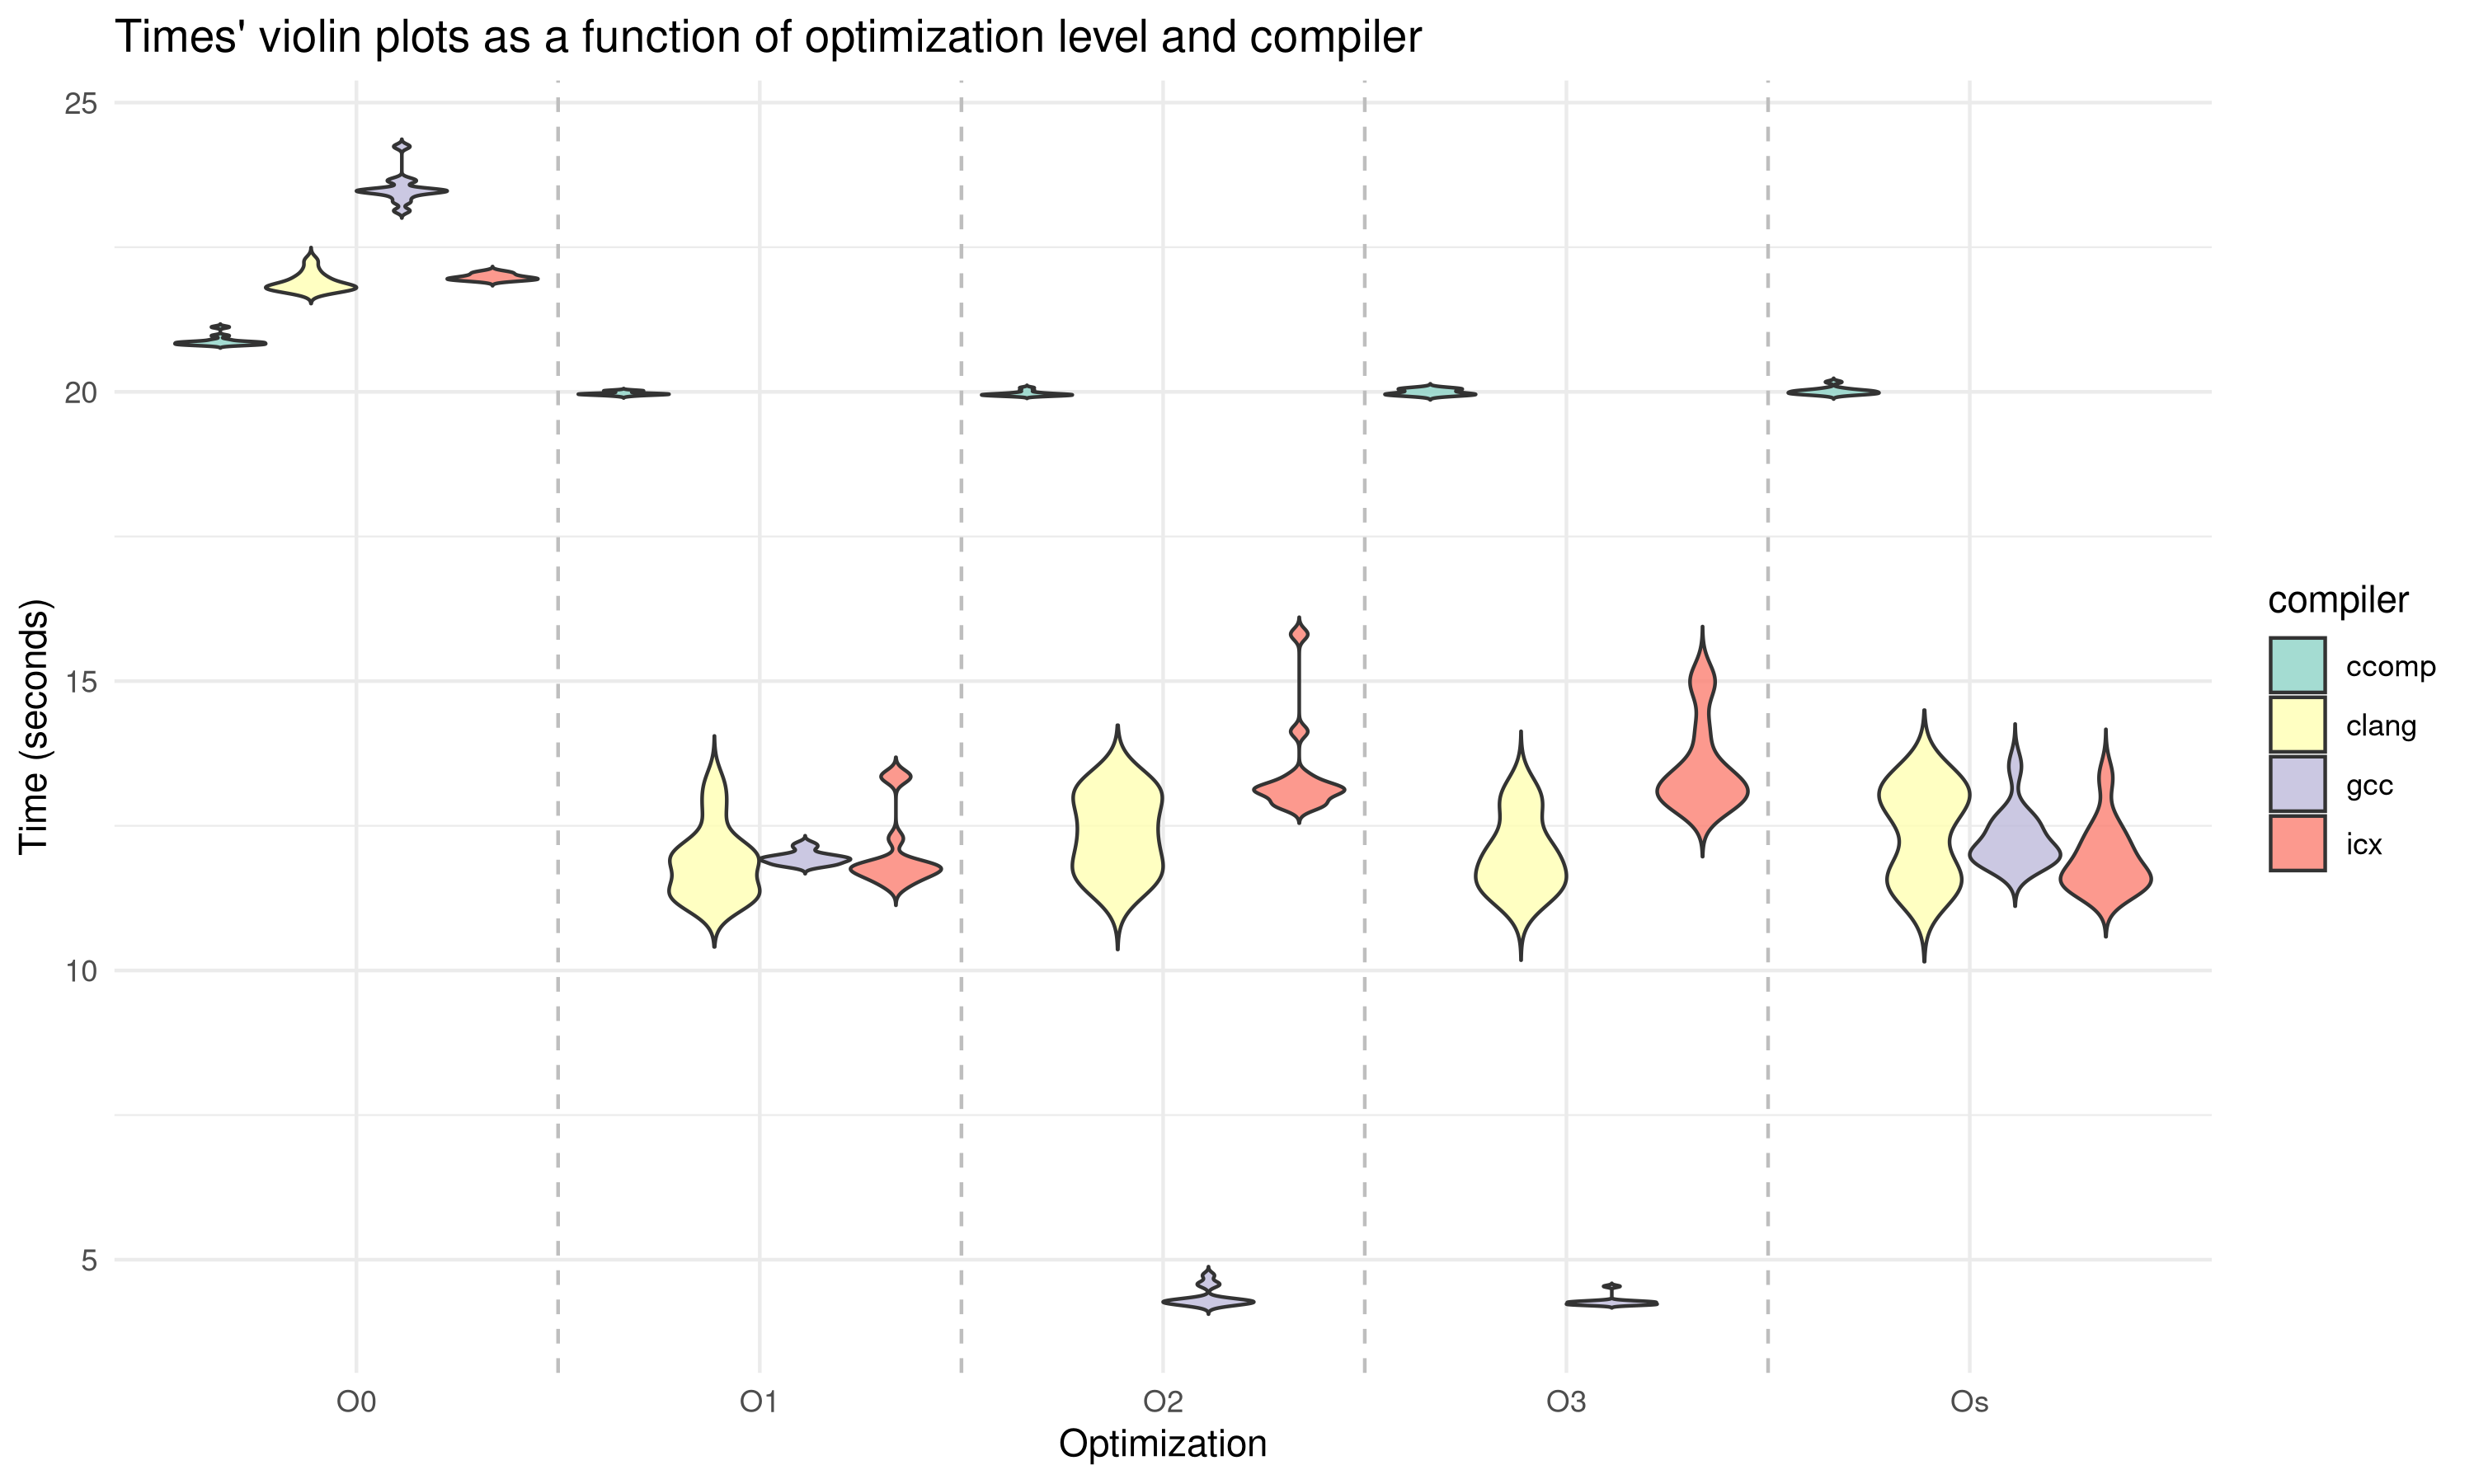
\includegraphics[width=1\textwidth]{img/plots/violin_plot_mat_mult.png}
    \caption{Evolution of the execution time of the program mat\_mult.c as a function of compiler and optimization level.}
    \label{fig:image1}
    \end{figure}
    \end{frame}
    
    \begin{frame}{Dijkstra Results}
    \begin{figure}[H]
    \centering
    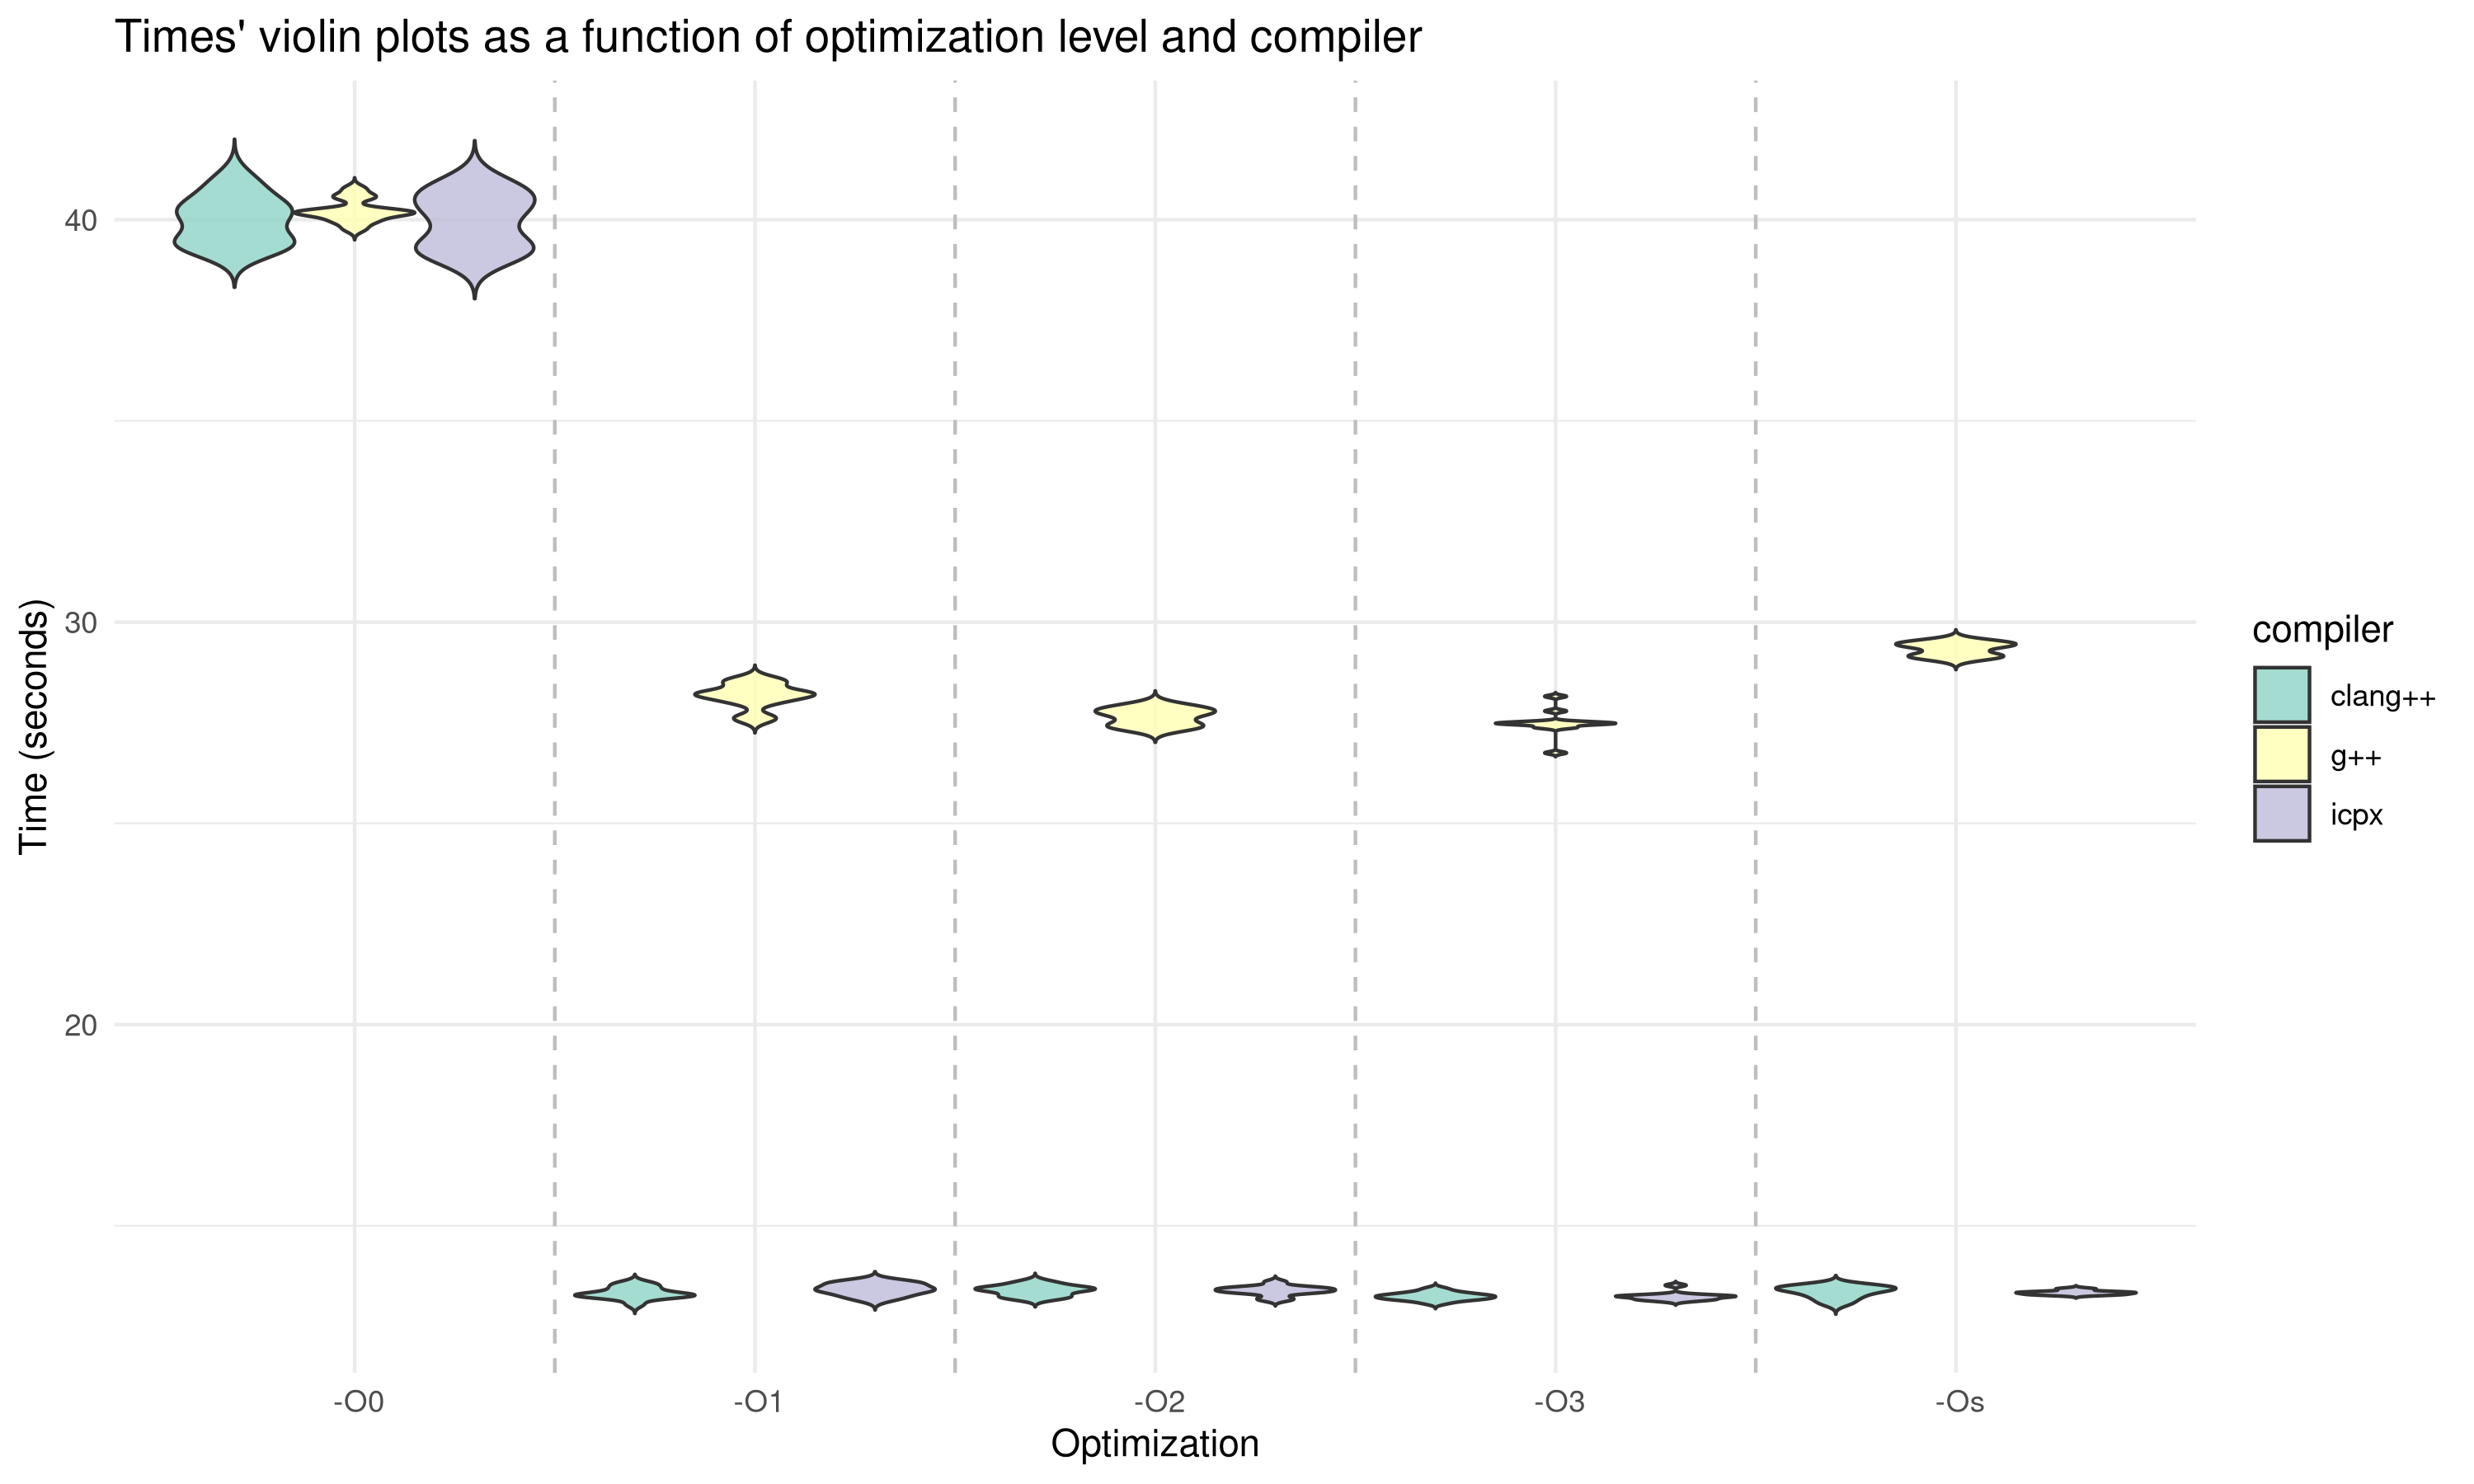
\includegraphics[width=1\textwidth]{img/plots/violin_plot_dijkstra.png}
    \caption{Evolution of the execution time of the program mat\_mult.c as a function of compiler and optimization level.}
    \label{fig:image2}
    \end{figure}
    \end{frame}
    
    
    \subsection{Matrix Multiplication}
    \subsection{Dijkstra}

\end{document}
